\documentclass[11pt,twocolumn]{article}
\usepackage{url}
\usepackage{breakurl}
\usepackage[breaklinks]{hyperref}
\usepackage{graphicx}
\usepackage{float}
\begin{document}

\begin{titlepage} % Suppresses displaying the page number on the title page and the subsequent page counts as page 1
    \newcommand{\HRule}{\rule{\linewidth}{0.5mm}} % Defines a new command for horizontal lines, change thickness here
    
    \center % Centre everything on the page
    
    %------------------------------------------------
    %    Headings
    %------------------------------------------------
    
    \textsc{\LARGE Indiana University - Bloomington}\\[1.5cm] % Main heading such as the name of your university/college
    
    \textsc{\Large Network Science}\\[0.5cm] % Major heading such as course name
        
    %------------------------------------------------
    %    Title
    %------------------------------------------------
    
    \HRule\\[0.4cm]
    
    {\huge\bfseries Measuring Facebook Influence Using Centrality Measures and Community Detection}\\[0.4cm] % Title of your document
    
    \HRule\\[1.5cm]
    
    %------------------------------------------------
    %    Author(s)
    %------------------------------------------------
    
    \begin{minipage}{0.4\textwidth}
        \begin{flushleft}
            \large
            \textit{Authors}\\
            \textsc{Daniel Hinders\newline} % Your name
            \textsc{Nhi Tran} % Your name

        \end{flushleft}


    \end{minipage}
    ~
    \begin{minipage}{0.4\textwidth}
        \begin{flushright}
            \large
            \textit{Professor}\\
            \textsc{Yong-Yeol (YY) Ahn} % Supervisor's name
        \end{flushright}
    \end{minipage}
    
    % If you don't want a supervisor, uncomment the two lines below and comment the code above
    %{\large\textit{Author}}\\
    %John \textsc{Smith} % Your name
    
    %------------------------------------------------
    %    Date
    %------------------------------------------------
    
    \vfill\vfill\vfill % Position the date 3/4 down the remaining page
    
    {\large\today} % Date, change the \today to a set date if you want to be precise
    
    %------------------------------------------------
    %    Logo
    %------------------------------------------------
    
    %\vfill\vfill
    %\includegraphics[width=0.2\textwidth]{placeholder.jpg}\\[1cm] % Include a department/university logo - this will require the graphicx package
     
    %----------------------------------------------------------------------------------------
    
    \vfill % Push the date up 1/4 of the remaining page
    
\end{titlepage}

\title{Measuring Facebook Influence Using Centrality Measures and Community Detection}
\author{Daniel Hinders and Nhi Tran}
\maketitle
\begin{abstract}
Within the past couple decades, social media has become a large part of everybody's life and our society. With the aid of social media, social influence can take place without physical human interaction and allow people to influence each other just by having social media accounts and the ability to access the Internet. After social media became popular, researchers and scientists have been studying the impact of social media using different methods such as surveys, trials, scientific experiments, and so on. Analyzing social media network graphs is another way of studying social media impact that this paper will cover. Given a public dataset of Page to Page network from Facebook in November 2017, multiple network graph measurements and a community detection method will help identify influential Fabebook pages within a network. By understanding the differences between measurements and what information they provide, it will be beneficial to apply similar measurements and analysis methods on other social media network to identify influential nodes.\end{abstract}

\section{Introduction}

With individuals having the ability to influence others anytime from any location anonymously, it is important to be able to identify their power and influential level within a social network to carefully access the impact. Without the ability to identify influential nodes, a network can be too large to study and time-consuming for anyone to get useful information.    


\subsection{Background}

Social media impact has drastically increased its effect on life in the last 10-15 years, the diverse and far reaching impacts cannot be overstated. Russian influence in the 2016 election, the Obama campaign utilizing social media to achieve a decisive victory in 2008 and social media fueling societal change and  upheaval in the middle east and Hong Kong are some of the examples. 

In another realm, corporations spend a massive 11.6 percent \cite{social-media-pricing} average of their marketing through social media indicating vast impact on societies choices and buying habits through social media.  

In the midst of these large organizations and vast movements in social media, there is a fascinating and powerful impact propagated through lone individuals on social media.  A single individual operating as a social media influencer is an existence that has become increasingly common in our societal vernacular. For many, a full time job as a social influencer has become a viable career. 

Understanding all of these social media forces and impacts is important on many levels. Devastating negative ramifications: a nation state subverting democracy by impacting other countries’ elections, hate groups spreading and inciting violence, and webs of misinformation leading to widespread distrust are all reasons alone to understand social media impact and influence. 

\subsection{Motivation and Objectives}

The ultimate purpose of this paper is to analyze a public Facebook Page-to-Page network to identify important nodes and different communities. 

The first objective is to answer the question that will observe the potential differences between multiple centrality measurements that help identify important nodes within a network - Can we simply use degree to identify powerful nodes in a network?


The second objective is to answer the question that will identify the different between a predetermined classification of a network and how likely would the nodes form a community within their own classification - Can we use page type to detect communities?




\subsection{Existing Work}

Social media is increasingly prevalent in commerce, politics, and all societal interaction. Unsurprising, research seeking to measure and understand social media influence and impact is prevalent. 
There are several studies that are related to our project objectives. Several use similar centrality measures and some community detection techniques. 


\paragraph{Existing Work 1 \cite{world-happiness-report-2018}} A Comparative Study of Modularity-Based Community Detection Methods for Online Social Networks 

http://ceur-ws.org/Vol-2201/UYMS_2018_paper_68.pdf	

Karatas & Sahin also focus on communities in social networks using modularity. The study assesses datasets from multiple social media platforms using different static community detection algorithms and specifically focus on “modularity values, running time and accuracy” and compare and contrast these different algorithms for community detection assessing their strengths and weaknesses. The performance of the different algorithms were analyzed by measuring their modularity value, F1-socre, and running time. Five different algorithms were used and the Louvain algorithm performed the best overall. The study suggests the following as problems with the current available community detection algorithms: stability, scalability, refinement on computational complexity, dynamicity, and prediction. These ideas prompt and encourage future research on community network structure and development of new community detection algorithms. 
   
\paragraph{Existing Work 2 \cite{world-happiness-report-2018}} Social Circles in Facebook communities

http://cseweb.ucsd.edu/classes/sp15/cse190-c/reports/sp15/022.pdf

The Social Circles in Facebook Communities study used the egonet dataset to assess specific subsets of the Facebook network which they termed social circles. Social circles are smaller groups within an individual’s social network such as friends from highschool or the workplace. The study utilized the egonet data set to construct various models of social circles and calculate Min Edit Distance and was purposed to: “predict what communities would form or what circles can be created using the given friendships” (Bansal, Anandan, & Techavatnavisal). Initially Clique Percolation to model the social circle data, but later in the study, the researchers found that Spectral Clustering was more effective. “Spectral Clustering is a way to cluster based on ‘Affinity’ and connectivity” (Bansal, Anandan, & Techavatnavisal). Our study perhaps is a logical partner and expansion on this study. In the future perhaps integrating these two concepts would benificatial. The incorporation influence assessment might be a beneficial step towards identifying how communities would form around influential nodes.

\paragraph{Existing Work 3 \cite{world-happiness-report-2018}} Network Analysis of Page Likes from Facebook User Profiles

https://ufdc.ufl.edu/UF00091523/00851

This study is unique because instead of analyzing social media network data where the nodes represent individuals connected to other individuals, they place Facebook pages representing companies instead of individuals as the nodes and connect them to people based upon page likes. Using the myPersonality application, Facebook pages with at least 100 likes were included as nodes and data was analyzed by calculation of clustering coefficient, diameter, and average path length. The study found that “the network’s in-degree distribution follows a power law” (Brauner, Kocheturov, & Pardalos). The conclusion of the study is that the structure of social media networks is consistent with small-world networks which are “characterized by dense local clustering and a short average path length between pairs of nodes” (Brauner, Kocheturov, & Pardalos)

\paragraph{Existing Work 4 \cite{world-happiness-report-2018}} Social Network Analysis with NetworkX

https://blog.dominodatalab.com/social-network-analysis-with-networkx/

This study used the Python library NetworkX to analyze network data from Facebook in graphic form. Using Facebook ego network which structures data along a central vertex, the exercise started by analyzing betweenness centrality to determine the most connected individuals present in the dataset. After calculating betweenness centrality, the highest scoring 10 in the dataset were placed as central hubs within the graph. Next different communities were identified using community detection algorithms focusing on the modularity of the network or the fraction of edges. 


\section{Process and Approaches}

\begin{figure}[hbt!]
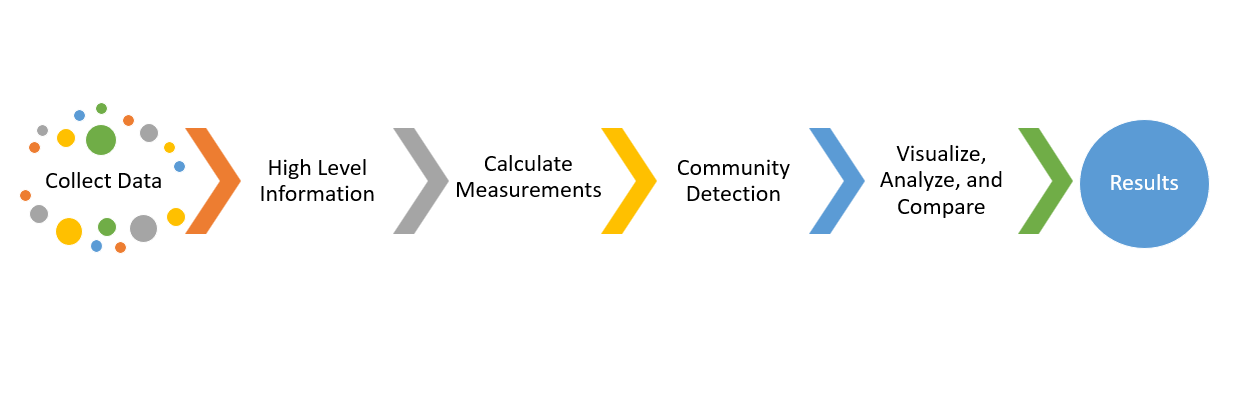
\includegraphics[scale=0.2]{process_flow.PNG} 
\caption{High Level Process}
\end{figure}

\textbf{Figure 1} identifies the steps that are necessary to complete the objectives of this report. Data are collected from Stanford Network Analysis Project. Once the data are collected, the next would be to clean up the network graph, perform high level analysis, calculations, detection community method. Then, all findings will be analyzed, visualized, and compared to get final results.

\subsection{Collecting Data}

\paragraph{Dataset \cite{page-page-network-ds}}
The dataset is November 2017 Facebook Large Page-Page Network from Stanford Network Analysis Project \cite{page-page-network-ds}. The dataset is a compressed zip file that contains the following files :
\begin{itemize}
\item\textbf{\texttt{musae\_facebook\_edges.csv}} – File that contains all edges between pages
\item\textbf{\texttt{musae\_facebook\_features.json}} – JSON file that contains features of the nodes - this file will not be used.
\item\textbf{\texttt{musae\_facebook\_target.csv}} - File that contains list of node ids, page names, and page types.
\end{itemize}

Each edge represents a mutual like between pages and each node is a Facebook page. There are four categories classifies for the Facebook pages: governmental organizations, politicians, television shows and companies. The raw data contains 22,470 nodes and 171,002 edges. 

\subsection{Data Cleaning and High Level Information}

\paragraph{Tools}
The following software and tools were used to perform the analysis:
\begin{itemize}
\item \textbf{Python and Python Packages} - Python packages include Networkx, Pandas, and Matplotlib
\item \textbf{Jupyter Notebook}
\item \textbf{Gephi} - visualization and analysis tool for network graph
\end{itemize}

\paragraph{Cleanup}
After using Pandas Python package to read and combine the edges list and pages categories information csv files, the next step would be converting the data into graph object and removing self-loops, edges that connect a node to itself. After removing self-loops, the total edge count reduced from 171,002 to 170,823.

\paragraph{High Level Information} 
The average degree is 15.2045, which means that on average, each node connects to about 15 other nodes. 

\begin{figure}[hbt!]
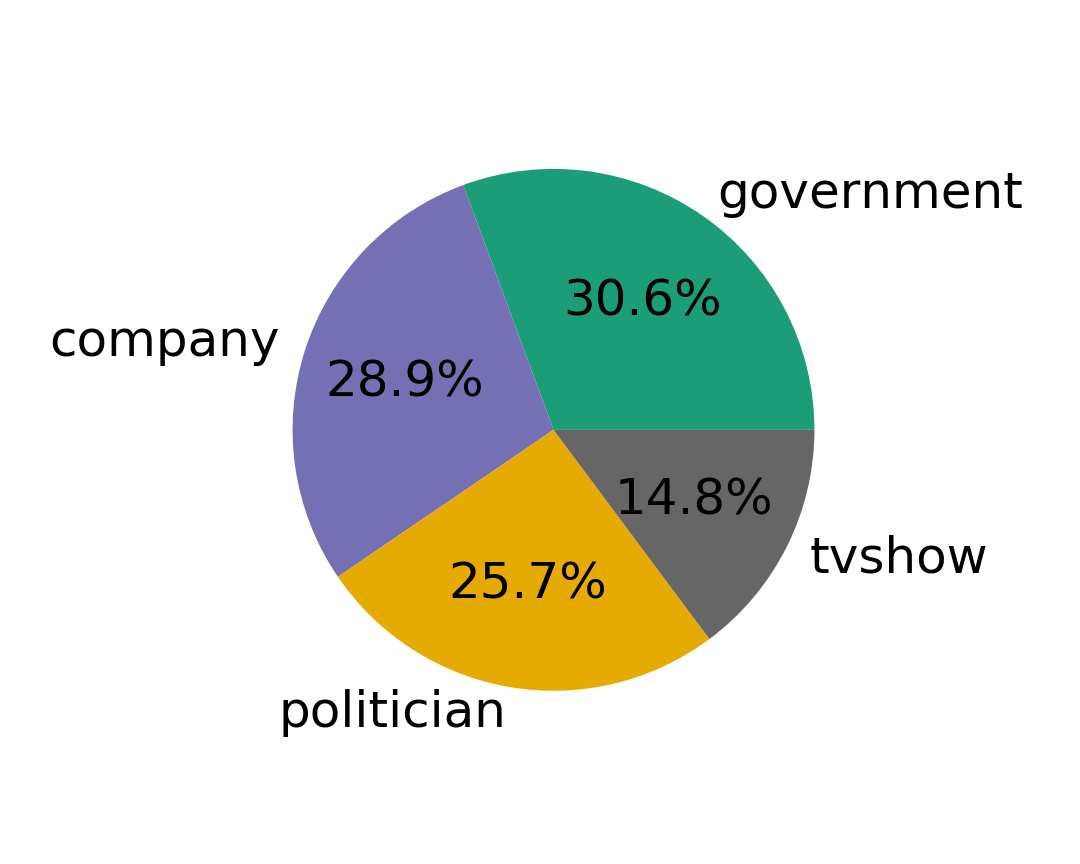
\includegraphics[scale=0.2]{pie_chart_category.png} 
\caption{Percentage of Page Category}
\end{figure}

\textbf{Figure 2} provides the composition of page category within the network.


\begin{figure}[hbt!]
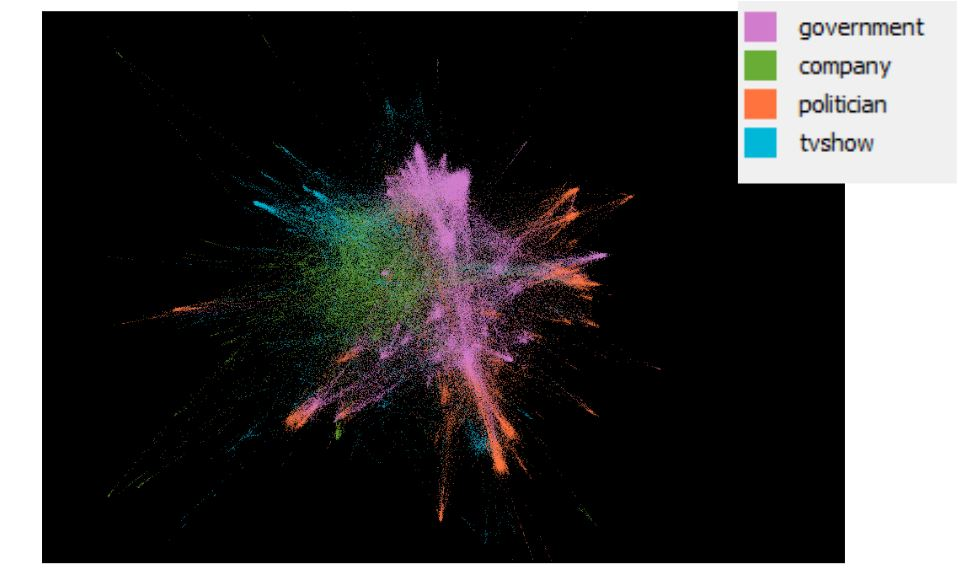
\includegraphics[scale=0.35]{gephi_whole_network_composition.JPG} 
\caption{Whole Network Visualization by Page Category}
\end{figure}


The same composition can be shown and visualized using Gephi as shown in \textbf{Figure 3}. One advantage of using Gephi over pie chart is the visual of clustered areas within a network. There is a highly connected area and some small clustered areas within governmental organization pages. Politicians and tv show pages also have more clustered area toward the outer part of the graph and Company pages don't have any obvious cluster. 

However, graphing the whole population makes it difficult to get more information out of the network. One way to workaround that is to filter the network into a smaller network of high degree nodes for more observations. By filtering the whole network to only select giant components with higher than 100 degree nodes, it resulted in a smaller network that only contains 314 nodes with 5,686 edges.


\begin{figure}[hbt!]
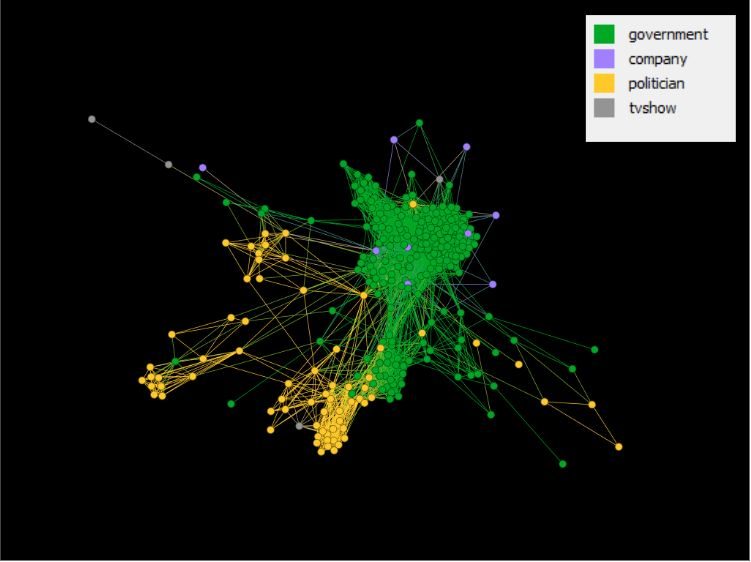
\includegraphics[scale=0.4]{gephi_filtered_100_degree.JPG} 
\caption{Visualization of Network with Nodes Greater Than 100 Degree}
\end{figure}

\textbf{Figure 4} shows that governmental organizations and politicians pages made of the majority of the population in a network of higher than 100 degree nodes. It is also quite easy to identify the cluster areas (about 5 areas).

Another high level measurement that is important and perhaps the most obvious measure of influence was a measurement of the degree of every node in the network. Degree centrality provides a simple yet telling quantitative data point for the number of edges or connections a given node has \cite{newman2008mathematics}.

\begin{figure}[hbt!]
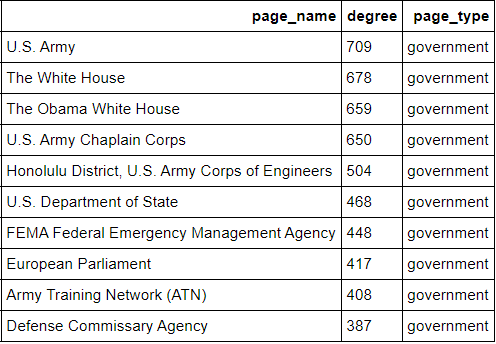
\includegraphics[scale=0.5]{top_ten_degree.png} 
\caption{Top Ten Highest Degree Pages}
\end{figure}

\textbf{Figure 5} contains the list of the top ten nodes that have the highest degree centrality within the whole network. One observation is that all of them are governmental organization pages; it aligns with the high composition of governmental organization pages shown in \textbf{Figure 4} earlier. It is interesting to see that the top five highest nodes are United State's related pages. Is it because the majority of Facebook users are in the United States or were the data skewed? Those are the questions that should be answered before making business or important decisions using this dataset.

\begin{figure}[hbt!]
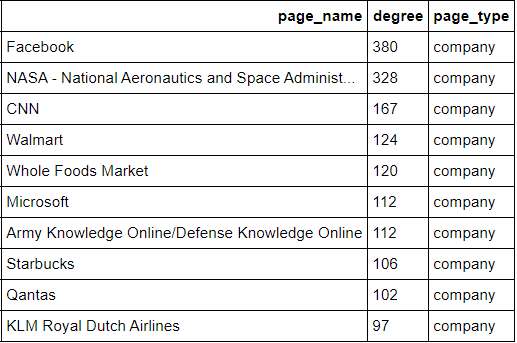
\includegraphics[scale=0.4]{top_ten_degree_company.png} 
\caption{Top Ten Highest Degree Company Pages}
\end{figure}
\begin{figure}[hbt!]
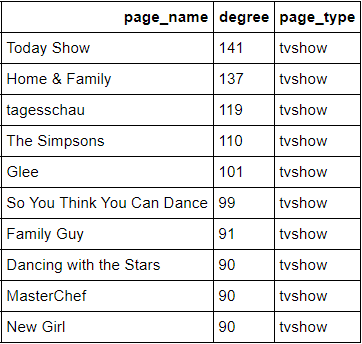
\includegraphics[scale=0.57]{top_ten_degree_tvshow.png} 
\caption{Top Ten Highest Degree TV Show Pages}
\end{figure}

\begin{figure}[hbt!]
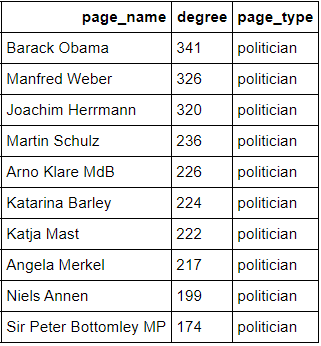
\includegraphics[scale=0.7]{top_ten_degree_politician.png} 
\caption{Top Ten Highest Degree Politician Pages}
\end{figure}


Additional filter of page type was added to get the top ten highest nodes of company pages, television shows, and politicians shown in \textbf{Figure 6}, \textbf{Figure 7}, and \textbf{Figure 8} respectively.  

Both of the top highest nodes under company and politician pages are about half of the degree amount comparing to the highest node in governmental organization. Television show pages seems to have the least influential power within this network.

\subsection{Calculate Measurements }
There are other centrality measurements that can be used to identify influential nodes within a network. It is important to understand the similarities and differences between these measurements and degree centrality to help with future network analysis. If degree centrality yields similar results to the rest of the other measurements, it might save time for researchers and scientists from having to calculate and perform deep-dive analysis.

\subsubsection{Betweenness Centrality} 
One of the useful centrality measurements to analyze a network is betweenness centrality. Betweenness centrality finds the path between every node in the network, then finds the shortest path and the nodes that fall into the most of these shortest paths will have the highest betweenness score \cite{newman2008mathematics}. 

\begin{figure}[hbt!]
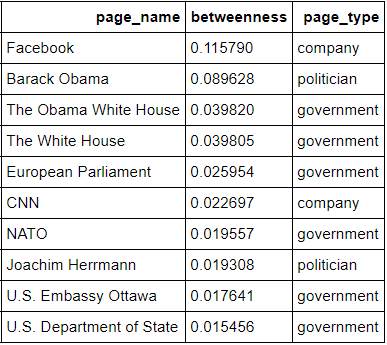
\includegraphics[scale=0.5]{top_ten_betweennness.png} 
\caption{Top Ten Highest Betweenness Centrality}
\end{figure}

\textbf{Figure 9} contains the top ten highests betweenness centrality nodes. The top ten nodes as calculated by their betweenness scores provides six governmental organization nodes, two politicians and two companies. The range of the scores is between 0.0155 for the 10th highest, and 0.116 for the 1st highest score.



\subsubsection{Closeness Centrality}
The next centrality measurement to analyze is closeness centrality. Closeness centrality provides the average path length between one node to every other vertex \cite{newman2008mathematics}.

\begin{figure}[hbt!]
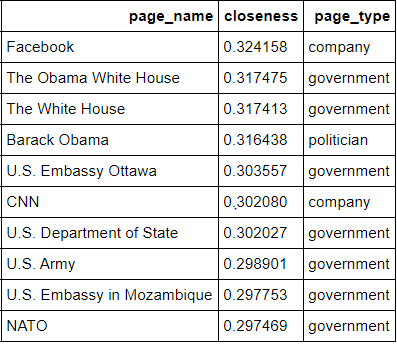
\includegraphics[scale=0.5]{top_ten_closeness.png} 
\caption{Top Ten Highest Closeness Centrality}
\end{figure}

\textbf{Figure 10} provided two companies, one politician, and seven governmental organizations in the top ten overall nodes with the highest Closeness centrality scores. The 10th highest had 0.0297 and the highest had 0.324.


\subsubsection{Eigenvector Centrality} 

Lastly, Eigenvector centrality need to be measured for this network. Eigenvector centrality measures the connections a node has, not just the quantity, but also the quality or the influence of those connected nodes. A high Eigenvector score would indicate that a node is connected to many other highly influential, high scoring nodes \cite{newman2008mathematics}. 
 
\begin{figure}[hbt!]
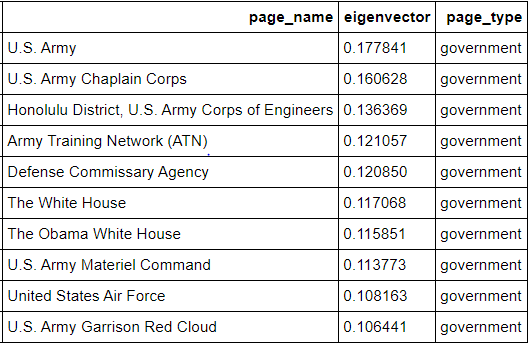
\includegraphics[scale=0.4]{top_ten_eigenvector.png} 
\caption{Top Ten Highest Eigenvector Centrality}
\end{figure}

Similar to degree, the top ten Eigenvector nodes are government related page types.  The range of the top ten eigenvector nodes ranges from 0.106 to 0.178 shown in \textbf{Figure 11}.

\subsection{Community Detection - Modularity}
The second objective evolves around the idea of community within a network and method to detect those communities. According to a research article called "Defining and Identifying Communities in Networks", a community is a group of nodes that have more dense connections  between themselves comparing to the rest of the network \cite{Radicchi2658}. One of the popular methods to detect community is by using Modularity measurement. Modularity is "the the portion of the edge connections within the same cluster minus the expected portion if the connections were distributed randomly" \cite{li_modular}.

Gephi can calculate and divide a network into each Modularity Class by providing a resolution number. According to Gephi's instruction, the higher the resolution value, the fewer the modularity classes there are. By passing a resolution value of 10, Gephi detected 8 modularity classes. 


\subsection{Visualize, Analyze and Compare}


\section{Discussion}


\section{Conclusion}


\section{Acknowledgment}
\section{References}
\bibliography{references} 
\bibliographystyle{ieeetr}
\end{document}
